% Created 2017-02-27 Mon 10:36
% Intended LaTeX compiler: pdflatex
\documentclass[a4paper,11pt]{article}
\usepackage[utf8]{inputenc}
\usepackage[T1]{fontenc}
\usepackage{graphicx}
\usepackage{grffile}
\usepackage{longtable}
\usepackage{wrapfig}
\usepackage{rotating}
\usepackage[normalem]{ulem}
\usepackage{amsmath}
\usepackage{textcomp}
\usepackage{amssymb}
\usepackage{capt-of}
\usepackage{hyperref}
\usepackage[margin=1in]{geometry}
\usepackage{setspace}
\onehalfspacing
\usepackage{parskip}
\usepackage{amsthm}
\usepackage{amsmath}
\usepackage{mathtools}
\usepackage{hyperref}
\usepackage{graphicx}
\usepackage{tabularx}
\usepackage{booktabs}
\hypersetup{colorlinks,citecolor=black,filecolor=black,linkcolor=black,urlcolor=black}
\newtheorem{definition}{Definition}
\newtheorem{theorem}{Theorem}
\newcommand{\rarrowd}[1]{\xrightarrow{\text{ \textit #1 }}}
\DeclareMathOperator*{\plim}{plim}
\newcommand{\plimn}{\plim_{n \rightarrow \infty}}
\setcounter{secnumdepth}{2}
\author{Zheng Tian}
\date{}
\title{Lecture 2: Review of Probability}
\hypersetup{
 pdfauthor={Zheng Tian},
 pdftitle={Lecture 2: Review of Probability},
 pdfkeywords={},
 pdfsubject={},
 pdfcreator={Emacs 25.1.1 (Org mode 9.0.3)}, 
 pdflang={English}}
\begin{document}

\maketitle
\setcounter{tocdepth}{2}
\tableofcontents

This lecture will review the basics in probability theory. The review
is by no means comprehensive. We will just refresh our mind with the
concepts that will be used the lectures that follow.

\section{Random Variables and Probability Distributions}
\label{sec:org45013ed}

\subsection{Defining probabilities and random variables}
\label{sec:orgd1b4cdf}

\subsubsection*{Experiments, outcomes, sample space, and events}
\label{sec:org9967528}

Probabilities are defined with respect to things whose occurrence are
random. We use the idea of an \textbf{experiment} to symbolize the processes
that generate random results. The \textbf{outcomes} of an experiment are its
mutually exclusive potential results. For example, a simple experiment
might be tossing a coin, the outcome of which is either getting a
head(H) or a tail(T) but not both.

We can denote all the outcomes from an experiment with a set \(S\), that
is called the \textbf{sample space}. In the tossing-coin experiment, the
sample space is \(\{H, T\}\). Or if we toss a dice, the sample space is
\(\{1, 2, 3, 4, 5, 6\}\). An \textbf{event} is a subset of the sample
space. Getting a head is an event, which is \(\{H\} \subset \{H, T\}\).

\subsubsection*{Probability}
\label{sec:org888c6a0}

The \textbf{probability} of an event is the proportion of the time that the
event will occur in the long run. For example, we toss a coin for \(n\)
times and get \(m\) heads. When \(n\) is very large, we can say that the
probability of getting a head in a toss is \(m/n\). Obviously, we cannot
always repeat an experiment with infinite times. So we need a general
(axiomatic) definition of probability as follows.

\subsubsection*{An axiomatic definition of probability}
\label{sec:orgb192625}

A probability of an event \(A\) in the sample space \(S\), denoted as
\(\mathrm{Pr}(A)\), is a function that assign \(A\) a real number in \([0,
1]\), satisfying the following three conditions:
\begin{enumerate}
\item \(0 \leq \mathrm{Pr}(A) \leq 1\).
\item \(\mathrm{Pr}(S) = 1\).
\item For any disjoint sets, \(A\) and \(B\), that is \(A\) and \(B\) have no
element in common, \(\mathrm{Pr}(A \cup B) = \mathrm{Pr}(A) +
  \mathrm{Pr}(B)\).
\end{enumerate}

Here we use the concept of disjoint (or mutually exclusive) sets. \(A\)
and \(B\) are disjoint if there is no common element between these two
sets, that is, \(A \cap B\) is an empty set.

\subsubsection*{Random variables}
\label{sec:orgc013f7a}

Instead of using words or a set symbol to represent an event or an
outcome, we can use numeric value to do so. A \textbf{random variable} is
thus a numerical summary associated with the outcomes of an
experiment. You can also think of a random variable as a function
mapping from an event \(\omega\) in the sample space \(\Omega\) to the
real line, as illustrated in Figure \ref{fig:org6d5a7bc}.

\begin{figure}[htbp]
\centering
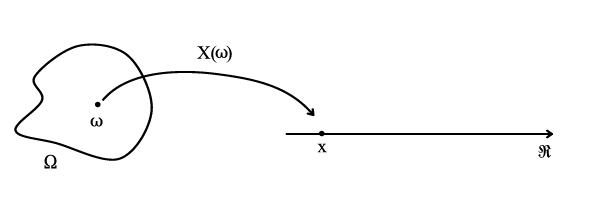
\includegraphics[width=0.8\textwidth]{figure/random_variable_demo1.png}
\caption{\label{fig:org6d5a7bc}
An illustration of random variable}
\end{figure}

Random variables can take different types of values. A \textbf{discrete} random
variables takes on a discrete set of values, like \(0, 1, 2, \ldots, n\)
whereas a \textbf{continuous} random variable takes on a continuum of possble
values, like any value in the interval \((a, b)\).


\subsection{Probability distributions}
\label{sec:org35f4a1f}

\subsubsection*{The probability distribution for a discrete random variable}
\label{sec:org3d102b0}

The probability distribution of a discrete random variable is the list
of all possible values of the variable and the probability that each
value will occur. These probabilities sum to 1.

\begin{itemize}
\item The probability mass function
\label{sec:org1559e62}

Let \(X\) be a discrete random variable. The probability distribution of
\(X\) (or the probability mass function), \(p(x)\), is
\begin{equation*}
p(x) = \mathrm{Pr}(X = x)
\end{equation*}
where we use \(X\) to denote the random variable and \(x\) to denote a
specific value that \(X\) can take. We denote the set of all possible
value of \(X\) as \(S\).

The axioms of probability require that (1) \(0 \leq p(x) \leq
1\) and (2) \(\sum_{i=1}^n p(x_i) = 1\).

\begin{table}[htbp]
\caption{\label{tab:orgaa4890a}
An illustration of the probability distribution of a discrete random variable}
\centering
\begin{tabular}{lrrrr}
\toprule
\(X\) & 1 & 2 & 3 & Sum\\
\midrule
\(\mathrm{P}(x)\) & 0.25 & 0.50 & 0.25 & 1.\\
\bottomrule
\end{tabular}
\end{table}

\item The cumulative probability distribution
\label{sec:org46f85dd}

The \textbf{cumulative probability distribution} (or the cumulative
distribution function, c.d.f.) is the probability that the random variable is
less than or equal to a particular value. Let \(F(x)\) be the c.d.f of
\(X\). Then \(F(x) = \mathrm{Pr}(X \leq x)\).

Table \ref{tab:orgc98c626} and Figure \ref{fig:org6534355} show that the
c.d.f. of a discrete random variable is a step function of \(x\).

\begin{table}[htbp]
\caption{\label{tab:orgc98c626}
An illustration of the c.d.f. of a discrete random variable}
\centering
\begin{tabular}{lrrrl}
\toprule
\(X\) & 1 & 2 & 3 & Sum\\
\midrule
\(\mathrm{P}(x)\) & 0.25 & 0.50 & 0.25 & 1\\
C.d.f. & 0.25 & 0.75 & 1 & --\\
\bottomrule
\end{tabular}
\end{table}

\begin{figure}[htbp]
\centering
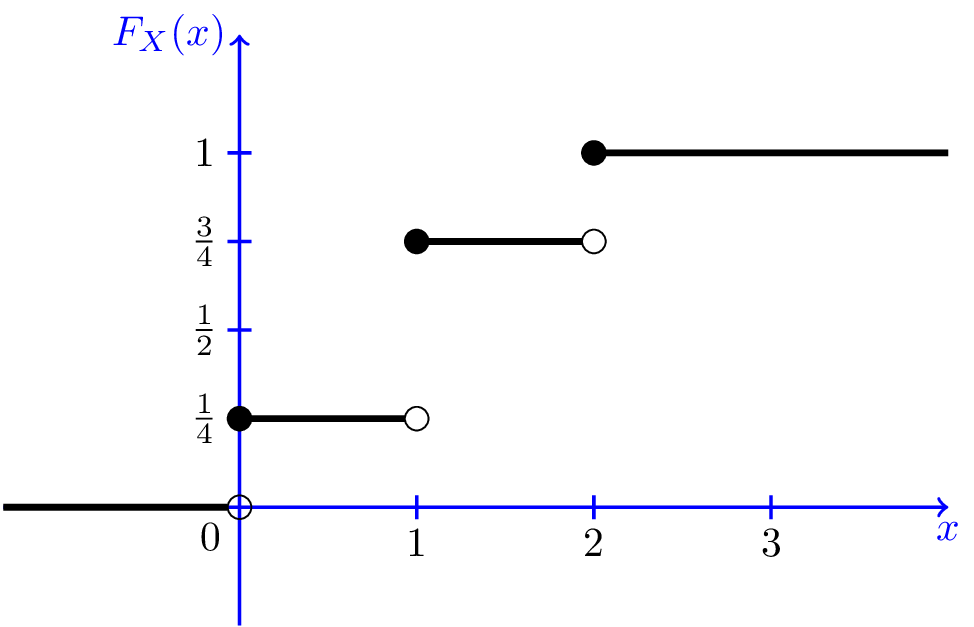
\includegraphics[width=0.53\textwidth,height=0.3\textheight]{figure/cdf_discrete_example.png}
\caption{\label{fig:org6534355}
The c.d.f. of a discrete random variable}
\end{figure}

\item Bernouli distribution
\label{sec:org04cde4c}

Many experiments like tossing a coin generate two outcomes: 1
with the probability of \(p\) and 0 with the probability of \(1-p\). The
random variable generated from such an experiment follows the Bernoulli
distribution.

The Bernoulli distribution
\begin{equation*}
  G =
    \begin{cases}
      1 & \text{with probability } p \\
      0 & \text{with probability } 1-p
    \end{cases}
  \end{equation*}
\end{itemize}

\subsubsection*{The probability distribution of a continuous random variable}
\label{sec:org1fb59c5}

Unlike a discrete random variable that we can enumerate its values for
each corresponding event, a specific value of a continuous random
variable is just a point in the real line, the probability of which is
zero. Instead, we use the concept of the \textbf{probability density function
(p.d.f)} as the counterpart of the probability mass function. And the
definition of the p.d.f. of a continuous random variable depends on
the definition of its. c.d.f.

The cumulative distribution function of a continous random variable
is defined as it is for a discrete random variable. That is, for a
continous random variable, \(X\), the c.d.f. is \(F(x) = \mathrm{Pr}(X
\leq x)\). And the \textbf{p.d.f.} of \(X\) is the function that satisfies
\[ F(x) = \int_{-\infty}^{x} f(t) \mathrm{d}t \text{ for all } x \]

\begin{figure}[htbp]
\centering
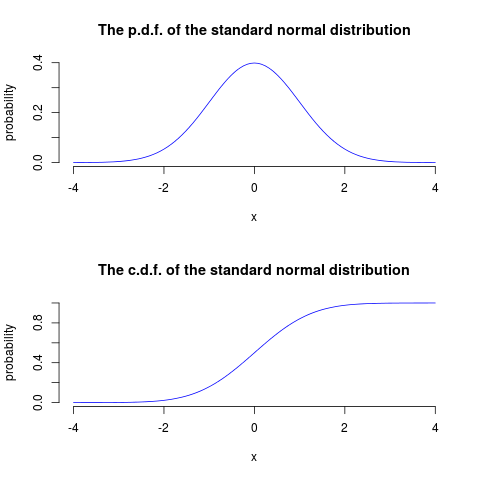
\includegraphics[width=0.6\textwidth,height=0.5\textheight]{figure/norm1.png}
\caption{\label{fig:org9899c28}
The p.d.f. and c.d.f. of a continuous random variable (the normal distribution)}
\end{figure}

For both discrete and continuous random variable, \(F(x)\) must satisfy
the following properties:
\begin{enumerate}
\item \(F(+\infty) = 1 \text{ and } F(-\infty) = 0\) (\(F(x)\) is bounded between 0 and 1)
\item \(x > y \Rightarrow F(x) \geq F(y)\) (\(F(x)\) is nondecreasing)
\end{enumerate}

By the definition of the c.d.f., we can conveniently calculate
probabilities, such as,
\begin{itemize}
\item \(\mathrm{P}(x > a) = 1 - \mathrm{P}(x \leq a) = 1 - F(a)\)
\item \(\mathrm{P}(a < x \leq b) = F(b) - F(a)\).
\end{itemize}

\textbf{A note on notation}. The c.d.f. and p.d.f. of a random variable \(X\) are
sometimes denoted as \(F_X(x)\) and \(f_X(x)\). In our lecture notes, if
there is no confusion, I will simply use \(F(x)\) and \(f(x)\) without the
subscript. 


\section{Expectation, Variance, and Other Moments}
\label{sec:org3558df2}

\subsection{The expected value of a random variable}
\label{sec:org7ffa4b7}

\subsubsection*{Definition}
\label{sec:org64fb606}

The \textbf{expected value} of a random variable, X, denoted as \(\mathrm{E}(X)\), is
the long-run average of the random variable over many repeated
trials or occurrences, which is also called the \textbf{expectation} or the
\textbf{mean}. The expected value measures the centrality of a random
variable.

\begin{itemize}
\item For a discrete random variable
\[ \mathrm{E}(X) = \sum_{i=1}^n x_i \mathrm{Pr}(X = x_i) \]

e.g. The expectation of a Bernoulli random variable, G
  \[ \mathrm{E}(G) = 1 \cdot p + 0 \cdot (1-p) = p \]

\item For a continuous random variable
\[ \mathrm{E}(X) = \int_{-\infty}^{\infty} x f(x) \mathrm{d}x\]
\end{itemize}

\subsection{The variance and standard deviation}
\label{sec:org773b9d7}

The \textbf{variance} of a random variable \(X\) measures its average
deviation from its own expected value. Let \(\mathrm{E}(X) = \mu_X\) and denote
the variance of \(X\), denoted as \(\mathrm{Var}(X)\) or \(\sigma^2_X\), is then

\begin{equation*}
\mathrm{Var}(X) = \mathrm{E}(X-\mu_X)^{2}=
\begin{cases}
\sum_{i=1}^n (x_i - \mu_X)^{2}\mathrm{Pr}(X = x_i) & \text{if } X \text{ is discrete} \\
\int_{-\infty}^{\infty} (x - \mu_X)^{2}f(x)\mathrm{d} x  & \text{if } X \text{ is continuous}
\end{cases}
\end{equation*}

The \textbf{standard deviation} of \(X\) is the square root of
\(\mathrm{Var}(X)\) and is denoted as \(\sigma_{X}\). That is,
\(\sigma_{X} = \sqrt{\mathrm{Var}(X)}\)

A convenient formula for calculating the variance is
\[ \mathrm{Var}(X) = \mathrm{E}(X - \mu_X)^{2} = \mathrm{E}(X^{2}) - \mu_X^{2} \]

The variance of a Bernoulli random variable, \(G\)
\[ \mathrm{Var}(G) = (1-p)^{2}p + (0-p)^{2}(1-p) = p(1-p) \] and \(\sigma_{G} =
\sqrt{p(1-p)}\).

From the definition of the expectation and variance, we can compute
the expectation and variance of a linear function of \(X\). Let \(Y = a +
bX\), then
\begin{itemize}
\item \(\mathrm{E}(Y) = a + b\mathrm{E}(X)\)
\item \(\mathrm{Var}(Y) = \mathrm{Var}(a + b X) = b^{2} \mathrm{Var}(X)\).
\end{itemize}


\subsection{Moments of a random variable, skewness and kurtosis}
\label{sec:orgd07caee}

The expectation and variance are two special cases of the \textbf{moments} of
a distribution.

\subsubsection*{Definition of the moments of a distribution}
\label{sec:org11d4633}

\begin{description}
\item[{k\(^{\text{th}}\) moment}] The k\(^{\text{th}}\) \textbf{moment} of the distribution of \(X\) is
\(\mathrm{E}(X^{k})\). So, the expectation is the "first"
moment of \(X\).

\item[{k\(^{\text{th}}\) central moment}] The k\(^{\text{th}}\) central moment of the distribution
of \(X\) with its mean \(\mu_X\) is \(\mathrm{E}(X - \mu_X)^{k}\). So, the
variance is the second central moment of \(X\).
\end{description}

It is important to remember that not all the moments of a distribution
exist. This is especially true for continuous random variables, for
which the integral to compute the moments may not converge.

\subsubsection*{Skewness and kurtosis}
\label{sec:org172cabe}

We also use the third and fourth central moments to measure how a
distribution looks like asymmetric and how thick are its tails.

\begin{itemize}
\item Skewness
\label{sec:org36cfa47}

The skewness of a distribution provides a mathematical way to describe
how much a distribution deviates from symmetry. It is defined as
\[ \text{Skewness} =  \mathrm{E}(X - \mu_X)^{3}/\sigma_{X}^{3} \]

\begin{itemize}
\item A symmetric distribution has a skewness of zero.
\item The skewness can be either positive or negative.
\item That \(\mathrm{E}(X - \mu_X)^3\) is divided by \(\sigma^3_X\) is to make the
skewness measure unit free. That is, changing the units of Y does
not change its skewness.
\end{itemize}

\item Kurtosis
\label{sec:org57b5a4a}

The kurtosis of the distribution of a random variable \(X\) measures how
much of the variance of \(X\) arises from extreme values, which makes
the distribution have "heavy" tails.

The kurtosis of the distribution of \(X\) is
\[ \text{Kurtosis} = \mathrm{E}(X - \mu_X)^{4}/\sigma_{X}^{4} \]

\begin{itemize}
\item The kurtosis must be positive.
\item The kurtosis of the normal distribution is 3. So a distribution that
has its kurtosis exceeding 3 is called heavy-tailed, or
\textbf{leptokurtic}.
\item The kurtosis is also unit free.
\end{itemize}

Figure \ref{fig:orgef50bf9} displays four distributions with different
skewness and kurtosis. All four distributions have a mean of zero and
a variance of one, while (a) and (b) are symmetric and (b)-(d) are
heavy-tailed.

\begin{figure}[htbp]
\centering
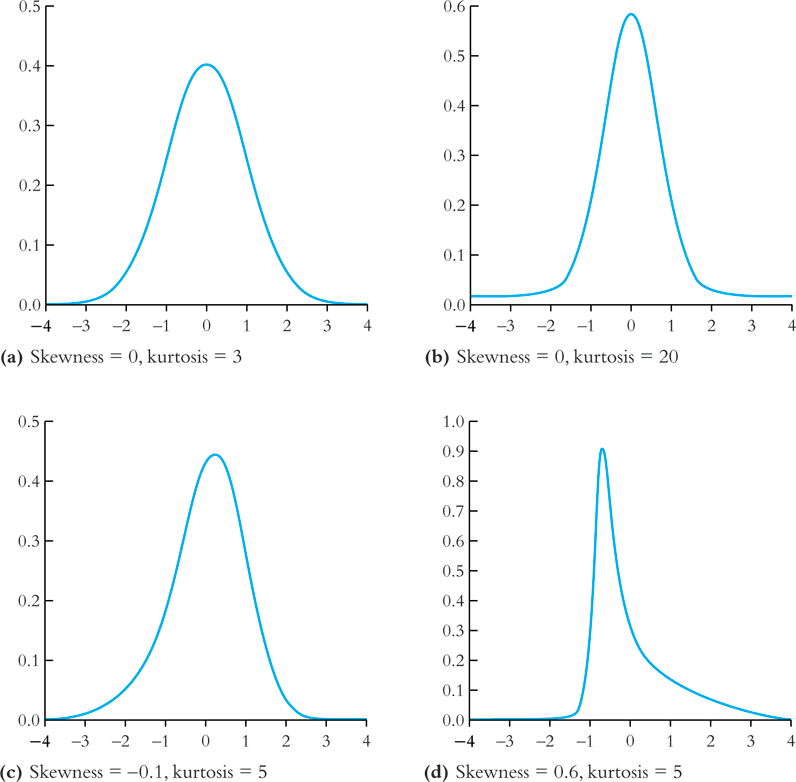
\includegraphics[width=0.75\textwidth,height=0.5\textheight]{figure/fig-2-3.png}
\caption{\label{fig:orgef50bf9}
Four distributions with different skewness and kurtosis}
\end{figure}
\end{itemize}


\section{Two Random Variables}
\label{sec:org7587253}

Econometrics in most cases considers the relations between two or
more variables. We use the concepts of joint, marginal, and
conditional distributions to describe such relations.

\subsection{The joint and marginal distributions}
\label{sec:orgdd0c6c6}

\subsubsection*{The joint probability functions}
\label{sec:org99927d4}

For two discrete random variables, \(X\) and \(Y\), the joint probability
distribution of \(X\) and \(Y\) is the probability that \(X\) and \(Y\)
simultaneously take on certain values, \(x\) and \(y\), that is
\[ p(x, y) = \mathrm{Pr}(X = x, Y = y)\]
which must satisfy the following
\begin{enumerate}
\item \(p(x, y) \geq 0\)
\item \(\sum_{i=1}^n\sum_{j=1}^m p(x_i, y_j) = 1\) for all possible
combinations of values of \(X\) and \(Y\).
\end{enumerate}

For two continuous random variables, \(X\) and \(Y\), the counterpart of \(p(x, y)\) is
the joint probability density function, \(f(x, y)\), such that
\begin{enumerate}
\item \(f(x, y) \geq 0\)
\item \(\int_{-\infty}^{{\infty}} \int_{-\infty}^{\infty} f(x, y)\, dx\, dy= 1\)
\end{enumerate}

\subsubsection*{The marginal probability distribution}
\label{sec:org3dc76d5}

The marginal probability distribution of a random variable \(X\) is
simply the probability distribution of its own. Since it is computed
from the joint probability distribution of \(X\) and \(Y\), we call it as
marginal probability of \(X\).

\begin{itemize}
\item For a discrete random variable, we can compute the marginal
distribution of \(X\) as
\[ \mathrm{Pr}(X=x) = \sum_{i=1}^n \mathrm{Pr}(X, Y=y_i) = \sum_{i=1}^n p(x, y_i)  \]
\item For a continuous random variable, the marginal distribution is
\[f_X(x) = \int_{-\infty}^{\infty} f(x, y)\, dy \]
\end{itemize}

By summing over or integrating out the values of \(Y\), we get the
probability distribution of \(X\) of its own.

\subsubsection*{An example of joint and marginal distributions}
\label{sec:org26ce88d}

Suppose we have two random variables: \(X\) and \(Y\). \(X\) equals 1 if
today is not raining and 0 otherwise, and \(Y\) equals 1 if it takes a short
time for commuting and 0 otherwise. The joint probability distribution
of these two random variables is the distribution that \(X\) takes the
value of 1 or 0 at the same time \(Y\) takes the value of 1 or 0, which
can be represented in the following table.

\begin{table}[htbp]
\caption{\label{tab:org40b74ef}
Joint distribution of raining and commuting time}
\centering
\begin{tabular}{lrrr}
 & Rain (\(X=0\)) & No rain (\(X=1\)) & Total\\
\hline
Long commute (\(Y=0\)) & 0.15 & 0.07 & 0.22\\
Short commute (\(Y=1\)) & 0.15 & 0.63 & 0.78\\
\hline
Total & 0.30 & 0.70 & 1\\
\end{tabular}
\end{table}

The four cells in the middle are the joint distribution. For example,
the joint probability of raining and taking a short commute is
0.15. The last row is the marginal distribution of \(X\), indicating
that the probability of raining no matter taking a long or short
commute is 0.30. The marginal distribution of \(X\) is in fact a
Bernoulli distribution. Similarly, the last column is the marginal
distribution of \(Y\), which is also a Bernoulli distribution.


\subsection{Conditional distributions}
\label{sec:org85885b7}

\subsubsection*{The conditional probability}
\label{sec:org78fe80f}

We often say that given one thing happens, what is the probability of
another thing to happen? To answer this question, we need the concept
of conditional probability.

For any two events \(A\) and \(B\), the conditional probability of A given
B is defined as
\begin{equation*}
\mathrm{Pr}(A|B) = \frac{\mathrm{Pr}(A \cap B)}{\mathrm{Pr}(B)}
\end{equation*}

Figure \ref{fig:org754fbfc}\footnote{Source of Figure \ref{fig:org754fbfc}: Pishro-Nik, Hossein. (2017). Introduction to
Probability \& Statistics. Retrieved from
\url{https://www.probabilitycourse.com/}.} helps us understand the
meaning of conditional probability. When we condition on the set B,
the sample space shrink from the original sample space, S, to a new
sample space, B. Since \(\mathrm{Pr}(A \cap B)\) is defined over S, so
we need to divide it by \(\mathrm{Pr}(B)\) to get \(\mathrm{Pr}(A|B)\).

\begin{figure}[htbp]
\centering
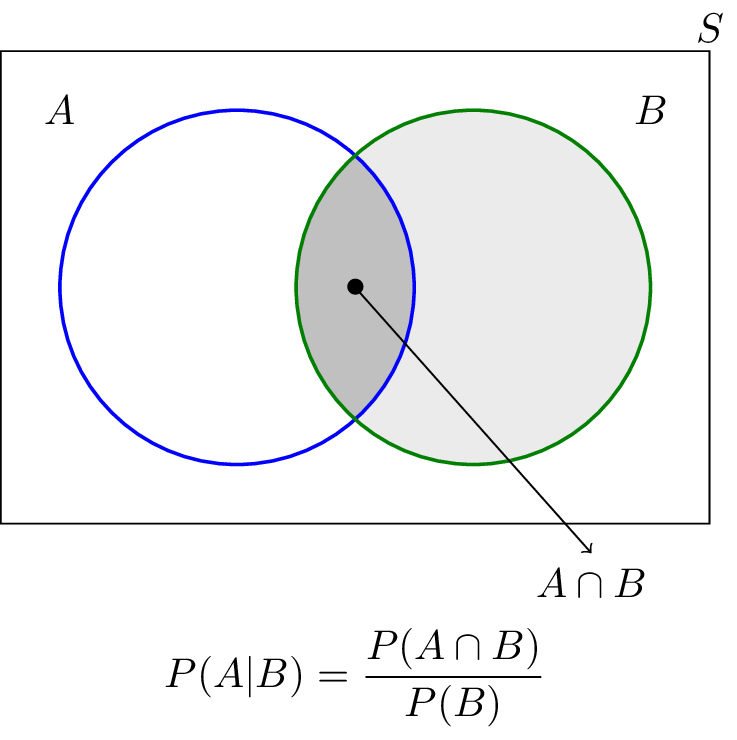
\includegraphics[width=0.45\textwidth,height=0.31\textheight]{figure/conditional_probability.png}
\caption{\label{fig:org754fbfc}
An illustration of conditional probability}
\end{figure}

\subsubsection*{The conditional probability distribution}
\label{sec:org99ada6e}

The conditional distribution of a random variable \(Y\) given another
random variable \(X\) is the distribution of \(Y\) conditional on X taking
a specific value, denoted as \(\mathrm{Pr}(Y | X=x)\). And the formula
to compute it is
\[ \mathrm{Pr}(Y | X=x) = \frac{\mathrm{Pr}(X=x,
Y)}{\mathrm{Pr}(X=x)} \]

For continuous random variables \(X\) and \(Y\), we define the conditional
density function as
\[ f(y|x) = \frac{f(x, y)}{f_X(x)} \]

In the above example of raining and commuting time, we can compute the
conditional distribution of commuting time given raining or not as
follows
\begin{center}
\begin{tabular}{llll}
\(\mathrm{Pr}(Y=0 \mid X=0)\) & 0.15/0.30 = 0.5 & \(\mathrm{Pr}(Y=0 \mid X=1)\) & 0.07/0.7 = 0.1\\
\(\mathrm{Pr}(Y=1 \mid X=0)\) & 0.15/0.30 = 0.5 & \(\mathrm{Pr}(Y=1 \mid X=1)\) & 0.63/0.7 = 0.9\\
\end{tabular}
\end{center}

\subsubsection*{The conditional expectation}
\label{sec:org3b99c00}

\begin{itemize}
\item Definition
\label{sec:org4aa22e7}

The \textbf{conditional expectation} of \(Y\) given \(X\) is the expected value
of the conditional distribution of \(Y\) given \(X\).

\begin{itemize}
\item For discrete random variables, the conditional mean of \(Y\) given \(X=x\) is
\begin{equation*}
\mathrm{E}(Y \mid X=x) = \sum_{i=1}^n y_i \mathrm{Pr}(Y=y_i \mid X=x)
\end{equation*}

\item For continuous random variables, it is computed as
\begin{equation*}
\int_{-\infty}^{\infty} y f(y \mid x)\, dy
\end{equation*}

\item The expected mean of commuting time given it is raining is \(0 \times
  0.1 + 1 \times 0.9 = 0.9\).
\end{itemize}

\item The law of iterated expectation
\label{sec:orga14f7e0}

Conditional expectations have a special property called \textbf{the law of
iterated expectation}, \(\mathrm{E}(Y) = E \left[ \mathrm{E}(Y|X) \right]\).

It says that the mean of \(Y\) is the weighted average of the
conditional expectation of \(Y\) given \(X\), weighted by the probability
distribution of \(X\). That is,
\[ \mathrm{E}(Y) = \sum_{i=1}^n \mathrm{E}(Y \mid X=x_i) \mathrm{Pr}(X=x_i) \]

The proof for the above equation is one question in the homework.

If \(\mathrm{E}(X|Y) = 0\), then \(\mathrm{E}(X)=E\left[\mathrm{E}(X|Y)\right]=0\).

\item Conditional variance
\label{sec:org504e8c8}

With the conditional mean of \(Y\) given \(X\), we can compute the
conditional variance as
\[ \mathrm{Var}(Y \mid X=x) = \sum_{i=1}^n \left[ y_i - \mathrm{E}(Y \mid X=x)
\right]^2 \mathrm{Pr}(Y=y_i \mid X=x) \]

From the law of iterated expectation, we can get the following
\[ \mathrm{Var}(Y) = \mathrm{E}(\mathrm{Var}(Y \mid X)) + \mathrm{Var}(\mathrm{E}(Y \mid
X)) \]
\end{itemize}

\subsubsection*{Independence}
\label{sec:org9a18c71}

\begin{itemize}
\item The definition of independent random variables
\label{sec:orgca7c4ba}

Two random variables \(X\) and \(Y\) are \textbf{independently distributed}, or
\textbf{independent}, if knowing the value of one of the variable provides no
information about the other. Mathematically, it means that 
\[ \mathrm{Pr}(Y=y \mid X=x) = \mathrm{Pr}(Y=y)  \]

It follows that if \(X\) and \(Y\) are independent
\[ \mathrm{Pr}(Y=y, X=x) = \mathrm{Pr}(X=x) \mathrm{Pr}(Y=y) \]

For two continuous random variables, \(X\) and \(Y\), they are
\textbf{independent} if
\[ f(x|y) = f_{X}(x) \text{ or } f(y|x) = f_{Y}(y) \]

It follows that if \(X\) and \(Y\) are independent
\[ f(x, y) = f(x|y)f_{Y}(y) = f_{X}(x)f_{Y}(y) \]
\end{itemize}


\subsection{Covariance and Correlation}
\label{sec:org3ad1265}

\subsubsection*{Covariance}
\label{sec:org366916c}

Covariance and correlation measure the co-movement of two random
variables. The covariance of two random variables \(X\) and \(Y\) is

\begin{align*}
\mathrm{Cov}(X, Y) & = \sigma_{XY} = \mathrm{E}(X-\mu_{X})(Y-\mu_{Y}) \\
                   & = \sum_{i=1}^n \sum_{j=1}^m (x_i - \mu_X)(y_j - \mu_Y) \mathrm{Pr}(X=x_i, Y=y_j)
\end{align*}

For continous random variables, the covariance of \(X\) and \(Y\) is
\[ \mathrm{Cov}(X, Y) = \int_{-\infty}^{\infty}
\int_{-\infty}^{\infty} (x-\mu_X)(y-\mu_y)f(x, y) dx dy \]

The covariance can also be computed as
\[ \mathrm{Cov}(X, Y) = \mathrm{E}(XY) - \mathrm{E}(X)\mathrm{E}(Y) \]

\subsubsection*{Correlation coefficient}
\label{sec:orgfbb9024}

Since the unit of the covariance of \(X\) and \(Y\) is the product of the
unit of \(X\) and that of \(Y\), its meaning is hard to be interpreted. We
often use the correlation coefficient to measure the correlation,
regardless of the units of \(X\) and \(Y\). The \textbf{correlation coefficient}
of \(X\) and \(Y\) is

\[ \mathrm{corr}(X, Y) = \rho_{XY} = \frac{\mathrm{Cov}(X, Y)}{\left[\mathrm{Var}(X)\mathrm{Var}(Y)\right]^{1/2}} =
\frac{\sigma_{XY}}{\sigma_{X}\sigma_{Y}} \]

The absolute value of a correlation coefficient must be less
than 1. That is, \(-1 \leq \mathrm{corr}(X, Y) \leq 1\). 

And \(\mathrm{corr}(X, Y)=0\) (or \(\mathrm{Cov}(X,Y)=0\)) means that \(X\)
and \(Y\) are uncorrelated. Since \(\mathrm{Cov}(X, Y) = \mathrm{E}(XY) -
\mathrm{E}(X)\mathrm{E}(Y)\), when \(X\) and \(Y\) are uncorrelated, then \(\mathrm{E}(XY) =
\mathrm{E}(X) \mathrm{E}(Y)\). 

\subsubsection*{Independence and uncorrelation}
\label{sec:org2b03471}

There is an important relationship between the two concepts of
independence and uncorrelation. If \(X\) and \(Y\) are independent, then

\begin{align*}
\mathrm{Cov}(X, Y) & = \sum_{i=1}^n \sum_{j=1}^m (x_i - \mu_X)(y_j - \mu_Y) \mathrm{Pr}(X=x_i) \mathrm{Pr}(Y=y_j) \\
                   & = \sum_{i=1}^n (x_i - \mu_X) \mathrm{Pr}(X=x_i) \sum_{j=1}^m (y_j - \mu_y) \mathrm{Pr}(Y=y_j) \\
                   & = 0 \times 0 = 0
\end{align*}

That is, if \(X\) and \(Y\) are independent, they must be
uncorrelated. However, the converse is not true. If \(X\) and \(Y\) are
uncorrelated, there is a possibility that they are actually
dependent. (Read this article, \href{http://www.stat.cmu.edu/\~cshalizi/uADA/13/reminders/uncorrelated-vs-independent.pdf}{``uncorrelated-vs-independent''}, for a detailed explanation\footnote{Shalizi, Cosma. (2013). Reminder No. 1: Uncorrelated
vs. Independent. Retrieved from
\url{http://www.stat.cmu.edu/\~cshalizi/uADA/13/reminders/uncorrelated-vs-independent.pdf}.})

Accordingly, if \(X\) and \(Y\) are independent, then we must have

\begin{align*}
\mathrm{E}(Y \mid X) & = \sum_{i=1}^n y_i \mathrm{Pr}(Y=y_i \mid X) \\
                     & = \sum_{i=1}^n y_i \mathrm{Pr}(Y=y_i) \\
                     & = \mathrm{E}(Y) = \mu_Y
\end{align*}

That is, the conditional mean of \(Y\) given \(X\) does not depend on any
value of \(X\) when \(Y\) is independent of \(X\). Then, we can prove that
\(\mathrm{Cov}(X, Y) = 0\) and \(\mathrm{corr}(X, Y)=0\).

\begin{align*}
\mathrm{E}(XY) & = \mathrm{E}(\mathrm{E}(XY \mid X)) = \mathrm{E}(X \mathrm{E}(Y \mid X)) \\
               & = \mathrm{E}(X) \mathrm{E}(Y \mid X) = \mathrm{E}(X) \mathrm{E}(Y)
\end{align*}

It follows that \(\mathrm{Cov}(X,Y) = \mathrm{E}(XY) - \mathrm{E}(X)
\mathrm{E}(Y) = 0\) and \(\mathrm{corr}(X, Y)=0\). 

Again, the converse is not true. That is, if \(X\) and \(Y\) are
uncorrelated, the conditional mean of \(Y\) given \(X\) may still depend
on \(X\). (See Exercise 2.23 at the end of Chapter 2.)

\subsubsection*{Some useful operations}
\label{sec:org69c6501}

Let \(X\) and \(Y\) be two random variables, with the means \(\mu_{X}\) and
\(\mu_{Y}\), the variance \(\sigma^{2}_{X}\) and \(\sigma^{2}_{Y}\), and the
covariance \(\sigma_{XY}\), respectively. Then, the following properties
of \(\mathrm{E}(\cdot)\), \(\mathrm{Var}(\cdot)\) and
\(\mathrm{Cov}(\cdot)\) are useful in calculation,

\begin{align*}
\mathrm{E}(a + bX + cY)      & = a + b \mu_{X} + c \mu_{Y} \\
\mathrm{Var}(aX + bY)        & = a^{2} \sigma^{2}_{X} + b^{2} \sigma^{2}_{Y} + 2ab\sigma_{XY} \\
\mathrm{Cov}(a + bX + cV, Y) & = b\sigma_{XY} + c\sigma_{VY} \\
\end{align*}


\section{Four Specific Distributions}
\label{sec:org666286c}

There are a variety of statistical distributions. In this course, we
will probably use the following four distributions: the normal
distribution, the chi-squared distribution, the student t
distribution, and the F distribution. 

\subsection{The normal distribution}
\label{sec:orgb746f03}

\subsubsection*{Definition}
\label{sec:orgd1f36b8}
The p.d.f. of a normally distributed random variable \(X\) is
\[ f(x) =
\frac{1}{\sigma\sqrt{2\pi}}\exp\left[-\frac{(x-\mu)^{2}}{2\sigma^{2}}\right]
\]
for which \(\mathrm{E}(X) = \mu\) and \(\mathrm{Var}(X) = \sigma^{2}\). We
usually write \(X \sim N(\mu, \sigma^{2})\) to say \(X\) has a normal
distribution with mean \(\mu\) and variance \(\sigma^2\). 

The standard normal distribution is a special case of the normal
distribution, for which \(\mu = 0\) and \(\sigma = 1\). The p.d.f of the
standard normal distribution is
\[
\phi(x) = \frac{1}{\sqrt{2\pi}}\exp\left(-\frac{x^2}{2}\right)
\]
The c.d.f of the standard normal distribution is often denoted as
\(\Phi(x)\).

The normal distribution is symmetric around its mean, \(\mu\), with the
skewness equal 0, and has 95\% of its probability between
\(\mu-1.96\sigma\) and \(\mu+1.96\sigma\), with the kurtosis
equal 3. Figure \ref{fig:org68e0e8c} displays the probability density of a
normal distribution.\footnote{Source of Figure \ref{fig:org68e0e8c}: Characteristics of the
Normal Distribution. Retrieved from
\url{http://howmed.net/community-medicine/normal-distribution-curve/}.}

\begin{figure}[htbp]
\centering
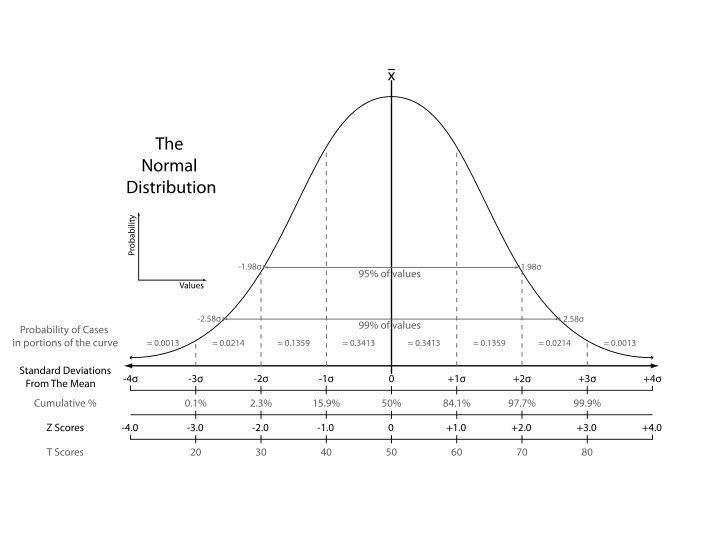
\includegraphics[width=0.9\textwidth]{figure/Normal-distribution-curve.png}
\caption{\label{fig:org68e0e8c}
The normal probability density}
\end{figure}

\subsubsection*{Transforming a normally distributed random variable to the standard normal distribution}
\label{sec:org0be4b9b}

Let \(X\) be a random variable with a normal distribution, i.e., \(X \sim
N(\mu, \sigma^2)\). Then, we can easily compute the probability of \(X\)
by transforming it into a random variable with the standard normal
distribution. We compute \(Z = (X-\mu)/\sigma\), which follows
the standard normal distribution, \(N(0, 1)\).

For example, if \(X \sim N(1, 4)\), then \(Z = (X-1)/2 \sim N(0,
1)\). When we want to find \(\mathrm{Pr}(X \leq 4)\), we only need to
compute \(\Phi(3/2)\).\footnote{The value of \(\Phi(x)\) can be found in a table for the standard
normal distribution, like the one in the following link,
\url{https://www.thestudentroom.co.uk/attachment.php?attachmentid=134337\&d=1330530156}.}

Generally, for any two number \(c_1 < c_2\) and let \(d_1 = (c_1 - \mu)/\sigma\) and
\(d_2 = (c_2 - \mu)/\sigma\), we have
\begin{align*}
\mathrm{Pr}(X \leq c_2) & = \mathrm{Pr}(Z \leq d_2) = \Phi(d_2) \\
\mathrm{Pr}(X \geq c_1) & = \mathrm{Pr}(Z \geq d_1) = 1 - \Phi(d_1) \\
\mathrm{Pr}(c_1 \leq X \leq c_2) & = \mathrm{Pr}(d_1 \leq Z \leq d_2) = \Phi(d_2) - \Phi(d_1)
\end{align*}

\subsubsection*{The multivariate normal distribution}
\label{sec:org091318f}

The normal distribution can be generalized to describe the joint
distribution of a set of random variables, which have the multivariate
normal distribution. (See Appendix 17.1 for the p.d.f of this
distribution and the special case of the bivariate normal
distribution.)

\begin{itemize}
\item Important properties of the multivariate normal distribution
\label{sec:org3947931}

\begin{enumerate}
\item If \(X\) and \(Y\) have a bivariate normal distribution with covariance
\(\sigma_{XY}\) and \(a\) and \(b\) are two constants, then
\[
   aX + bY \sim N(a\mu_X + b\mu_Y, a^2\sigma_X + b^2\sigma_Y +
   2ab\sigma_{XY})
   \]

More generally, if n random variables, \(x_1, \ldots, x_n\), have a
multivariate normal distribution, then any linear combination of
these variables is normally distributed, for example, \(\sum_{i=1}^n
   x_i\). For any real numbers, \(\alpha_1, \ldots, \alpha_n\), a linear
combination of \({x_i}\) is \(\sum_i \alpha_i x_i\).

\item If a set of random variables has a multivariate normal
distribution, then the marginal distribution of each of the
variables is normal.

\item If random variables with a multivariate normal distribution have
covariances that equal zero, then these random variables are
independent.

Let \(X\) and \(Y\) be two random variables with a bivariate normal
distribution. The joint p.d.f of \(X\) and \(Y\) is \(f(x, y)\), with the
marginal p.d.f. being \(f_X(x)\) and \(f_Y(y)\), respectively. Then we have
\[ \mathrm{Cov}(X, Y) = 0 \Leftrightarrow f(x, y) = f_X(x)f_Y(y) \]

\textbf{Note}: this property only holds for random variables with a
multivariate normal distribution. Generally, uncorrelation does not
imply independence.

\item If \(X\) and \(Y\) have a bivariate normal distribution, then
\[\mathrm{E}(Y|X = x) = a + bx \]
where \(a\) and \(b\) are constants.
\end{enumerate}
\end{itemize}


\subsection{The chi-squared distribution}
\label{sec:orga57307a}

Let \(Z_1, \ldots, Z_n\) be n indepenent standard normal distribution,
i.e. \(Z_i \sim N(0, 1)\) for all \(i = 1, \ldots, n\). Then, the random
variable
\[W = \sum_{i=1}^n Z^2_i \]
has a chi-squared distribution with \(n\) degrees of freedom, denoted as
\(W \sim \chi^2(n)\), with \(\mathrm{E}(W) = n\) and \(\mathrm{Var}(W) = 2n\)

If \(Z \sim N(0, 1)\), then \(W = Z^2 \sim \chi^2(1)\) with \(\mathrm{E}(W) =
1\) and \(\mathrm{Var}(W) = 2\).

Figure \ref{fig:orgb305124} shows the p.d.f. of chi-squared distributions
with different degrees of freedom. 

\begin{figure}[htbp]
\centering
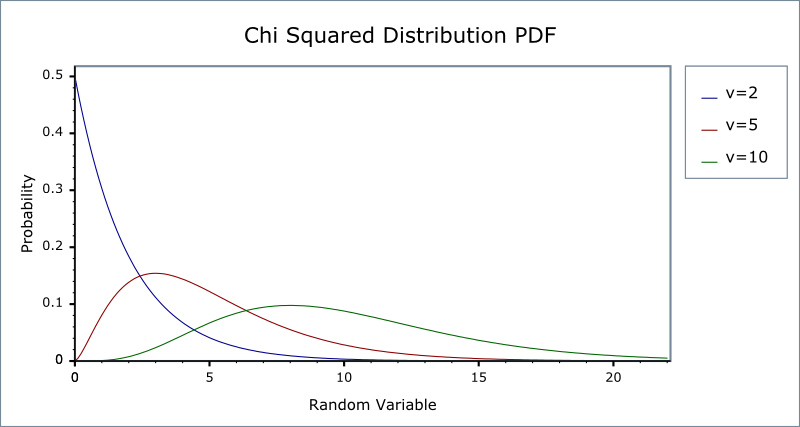
\includegraphics[width=0.8\textwidth]{figure/chi_squared_pdf.png}
\caption{\label{fig:orgb305124}
The probability density function of chi-squared distributions}
\end{figure}


\subsection{The student t distribution}
\label{sec:org1c27cf8}

Let \(Z \sim N(0, 1)\), \(W \sim \chi^2(m)\), and \(Z\) and \(W\) be
independently distributed. Then, the random variable
\[t = \frac{Z}{\sqrt{W/m}} \]
has a student t distribution with \(m\) degrees of freedom, denoted as
\(t \sim t(m)\).

As \(n\) increases, \(t\) gets close to a standard normal distribution.

Figure \ref{fig:org55e2339} shows the p.d.f. of student t distributions
with different degrees of freedom. 

\begin{figure}[htbp]
\centering
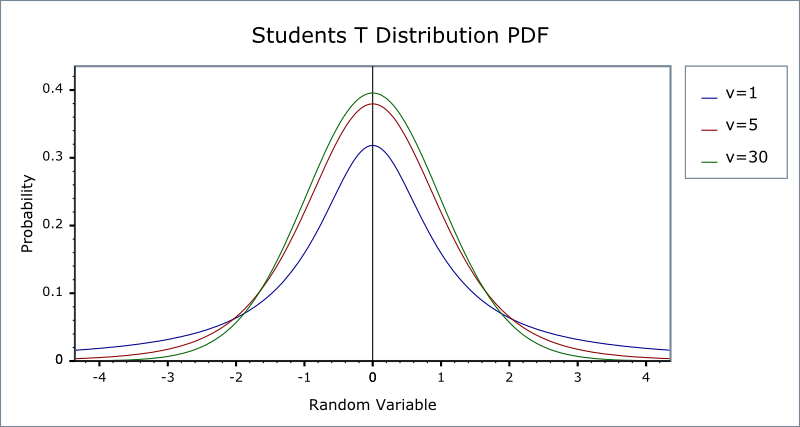
\includegraphics[width=0.8\textwidth]{figure/students_t_pdf.png}
\caption{\label{fig:org55e2339}
The probability density function of student t distributions}
\end{figure}


\subsection{The F distribution}
\label{sec:org0491dbd}

Let \(W_1 \sim \chi^2(n_1)\), \(W_2 \sim \chi^2(n_2)\), and \(W_1\) and
\(W_2\) are independent. Then, the random variable
\[ F = \frac{W_1/n_1}{W_2/n_2}\]
has an F distribution with \((n_1, n_2)\) degrees of freedom, denoted as
\(F \sim F(n_1, n_2)\)

\begin{itemize}
\item If \(t \sim t(n)\), then \(t^2 \sim F(1, n)\)
\item As \(n_2 \rightarrow \infty\), the \(F(n_1, \infty)\) distribution is the
same as the \(\chi^2(n_1)\) distribution divided by \(n_1\).
\end{itemize}

Figure \ref{fig:org37f1740} shows the p.d.f. of F distributions
with different degrees of freedom. 

\begin{figure}[htbp]
\centering
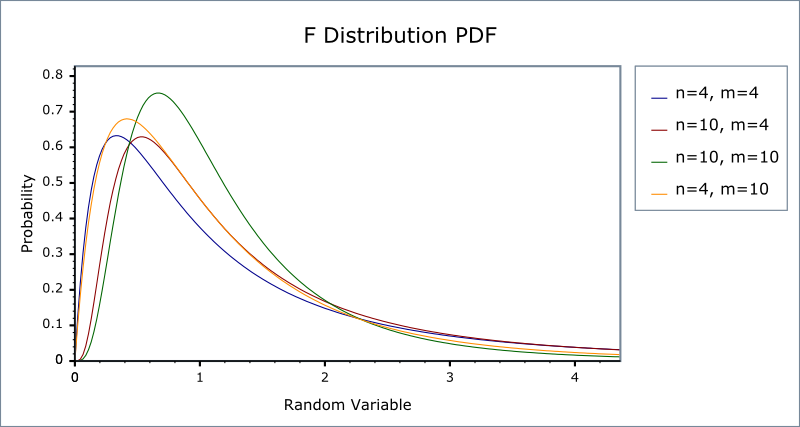
\includegraphics[width=0.8\textwidth]{figure/fisher_f_pdf.png}
\caption{\label{fig:org37f1740}
The probability density function of F distributions}
\end{figure}


\section{Random Sampling and the Distribution of the Sample Average}
\label{sec:orgce32373}

\subsection{Random sampling}
\label{sec:orgaadfa7d}

Almost all the statistical and econometric procedures involve averages
of a sample of data. When samples are randomly drawn from a larger
population, the average itself is a random variable. Therefore, in
the next three sections, we consider the distributions of sample
averages. 

\subsubsection*{Simple random sampling}
\label{sec:org471cd68}

In statistics, a \textbf{population} is a set of similar items or events which
is of interest for some question or experiment. A statistical
population can be a group of actually existing objects (e.g. the set
of all stars within the Milky Way galaxy) or a hypothetical and
potentially infinite group of objects conceived as a generalization
from experience (e.g. the set of all possible hands in a game of
poker).\footnote{Wikipedia. Statistical population. Retrieved from
\url{https://en.wikipedia.org/wiki/Statistical\_population}.}

\textbf{Simple random sampling} is a procedure in which \(n\) objects are
selected at random from a population, and each member of the
population is equally likely to be included in the sample. 

Let \(Y_1, Y_2, \ldots Y_n\) be the first \(n\) observations in a random
sample. Since they are randomly drawn from a population, \(Y_1, \ldots,
Y_n\) are random variables. And the sample average is also a random
variable. 

\subsubsection*{i.i.d draws}
\label{sec:org1c0add8}

Since \(Y_1, Y_2, \ldots, Y_n\) are drawn from the same population, the
marginal distribution of \(Y_i\) is the same for each \(i=1, \ldots,
n\). And the marginal distribution is the distribution of the
population \(Y\). When \(Y_i\) has the same marginal distribution for
\(i=1, \ldots, n\), then \(Y_1, \ldots, Y_n\) are said to be \textbf{identically
distributed}. 

With simple random sampling, the value of \(Y_i\) does not depend on
that of \(Y_j\) for \(i \neq j\). That is, under simple random sampling,
\(Y_1, \ldots, Y_n\) are \textbf{independent distributed}. 

Therefore, when \(Y_1, \ldots, Y_n\) are drawn with simple random
sampling from the same distribution of \(Y\), we say that they are
\textbf{independently and identically distributed} or \textbf{i.i.d}, which can be
denoted as 
\[ Y_i \sim IID(\mu_Y, \sigma^2_Y) \text{ for } i = 1, 2, \ldots, n\]
given that the population expectation is \(\mu_Y\) and the variance
is \(\sigma^2_Y\).


\subsection{The sampling distribution of the sample average}
\label{sec:org60e2753}

\subsubsection*{The sample average}
\label{sec:orgd663703}

The \textbf{sample average} or \textbf{sample mean}, \(\overline{Y}\), of the \(n\)
observations \(Y_1, Y_2, \ldots, Y_n\) is
\[ \overline{Y} = \frac{1}{n}\sum^n_{i=1} Y_i \]

When \(Y_1, \ldots, Y_n\) are randomly drawn, \(\overline{Y}\) is also a
random variable that should have its own distribution, called the
\textbf{sampling distribution}. We are mostly interested in the mean,
variance, and the form of the sampling distribution.

\subsubsection*{The mean and variance of \(\overline{Y}\)}
\label{sec:org57bc4ac}

Suppose that \(Y_i \sim IID(\mu_Y, \sigma^2_{Y})\) for all \(i = 1,
\ldots, n\). Then, by the definition of \(\overline{Y}\) and the fact
that \(Y_i\) and \(Y_j\) are independent for any \(i \neq j\) and thus,
\(\mathrm{Cov}(Y_i, Y_j)=0\), we have
\[
\mathrm{E}(\overline{Y}) = \mu_{\overline{Y}} =
\frac{1}{n}\sum^n_{i=1}\mathrm{E}(Y_i) = \frac{1}{n} n \mu_Y = \mu_Y
\]
and
\[
\mathrm{Var}(\overline{Y}) = \sigma^2_{\overline{Y}} =  \frac{1}{n^2}\sum^n_{i=1}\mathrm{Var}(Y_i) +
\frac{1}{n^2}\sum^n_{i=1}\sum^n_{j=1}\mathrm{Cov}(Y_i, Y_j) =
\frac{\sigma^2_Y}{n}
\]
And the standard deviation of the sample mean is
\(\sigma_{\overline{Y}} = \sigma_Y / \sqrt{n}\).

\subsubsection*{Sampling distribution of \(\overline{Y}\) when \(Y\) is normally distributed}
\label{sec:org0143aea}

The sample average \(\overline{Y}\) is a linear combination of \(Y_1,
\ldots, Y_n\). When \(Y_1, \ldots, Y_n\) are i.i.d. draws from \(N(\mu_Y,
\sigma^2_Y)\), from the properties of the multivariate normal
distribution, \(\overline{Y}\) is normally distributed. That is 
\[ \overline{Y} \sim N(\mu_Y, \sigma^2_Y/n) \]


\section{Large Sample Approximations to Sampling Distributions}
\label{sec:org9aa2d40}

\subsection{The exact distribution and the asymptotic distribution}
\label{sec:org5617959}

The sampling distribution that exactly describes the distribution of
\(\overline{Y}\) for any \(n\) is called the \textbf{exact distribution} or
\textbf{finite-sample distribution}. For example, when \(Y\) is normally
distributed and \(Y_1, \ldots, Y_n\) are i.i.d. draws from \(N(\mu_Y,
\sigma^2_Y)\), we know the exact distribution of \(\overline{Y}\) is
\(N(\mu_Y, \sigma^2_Y/n)\). 

However, in most cases, we cannot obtain an exact distribution of
\(\overline{Y}\), for which we can only get an approximation. The
large-sample approximation to the sampling distribution is called the
\textbf{asymptotic distribution}. The existence of the asymptotic
distribution of \(\overline{Y}\) is guaranteed by the \textbf{law of large
numbers} and the \textbf{central limit theorem}. 


\subsection{The law of large numbers}
\label{sec:orgd6af81c}

\subsubsection*{Convergence in probability}
\label{sec:org9b07f3d}

Let \(S_1, \ldots, S_n\) be a sequence of random variables,
denoted as \(\{S_n\}\). \(\{S_n\}\) is said to converge in probability to a
limit \(\mu\) (denoted as \(S_n \xrightarrow{\text{p}} \mu\)), if and only if
\[ \mathrm{Pr} \left(|S_n-\mu| < \delta \right) \rightarrow 1 \]
as \(n \rightarrow \infty\) for every \(\delta > 0\).

For example, \(S_n = \overline{Y}\). That is, \(S_1=Y_1\), \(S_2=1/2(Y_1+Y_2)\),
\(S_n=1/n\sum_i Y_i\), and so forth.

\subsubsection*{The law of large numbers}
\label{sec:org9f18dec}

The law of large numbers (LLN) states that if \(Y_1, \ldots, Y_n\) are i.i.d. with
\(\mathrm{E}(Y_i)=\mu_Y\) and \(\mathrm{Var}(Y_i) < \infty\), then
\(\overline{Y} \xrightarrow{\text{p}} \mu_Y\). 

The conditions for the LLN to be held is \(Y_i\) for \(i=1, \ldots, n\)
are i.i.d., and the variance of \(Y_i\) is finite. The latter says that
there is no extremely large outliers in the random samples. The
presence of outliers in the sample can substantially influence the
sample mean, rendering its convergence to be unachievable. 

Figure \ref{fig:org6610dba} shows that the convergence sample mean of random
samples from a Bernoulli distribution that \(\mathrm{Pr}(Y_i = 1) =
0.78\). As the number of sample increases, the sample mean (i.e., the
proportion that \(Y_i = 1\)) get close to the true mean of 0.78. 

\begin{figure}[htbp]
\centering
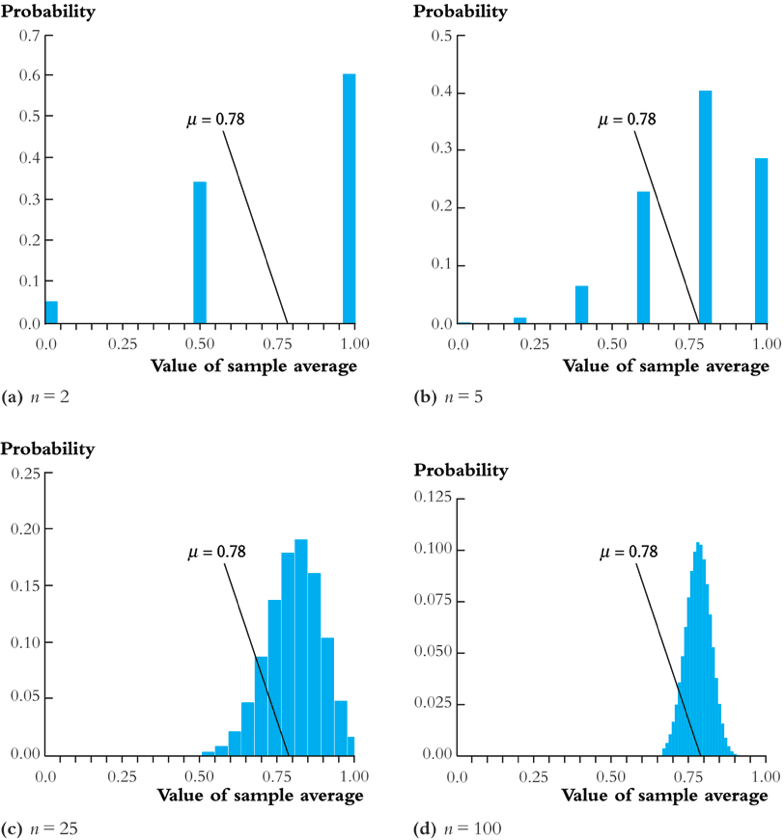
\includegraphics[width=0.75\textwidth]{figure/fig-2-8.png}
\caption{\label{fig:org6610dba}
An illustration of the law of large numbers}
\end{figure}

Here is another demonstration of the law of large number,\footnote{This example and the one for the CLT are both retrieved from
\url{http://demonstrations.wolfram.com/index.html}.}
\url{IllustratingTheLawOfLargeNumbers.cdf}. To view this file,
first you need to download them by saving into your disk, then open
them with Wolfram CDF Player that can be downloaded from
\url{http://www.wolfram.com/cdf-player/}.


\subsection{The central limit theorem}
\label{sec:org1597dea}

The LLN ensures the convergence of the sample mean from the sampling
distribution, while the \textbf{central limit theorem} (CLT) ensures the
convergence of the sampling distribution itself. 

\subsubsection*{Convergence in distribution}
\label{sec:org1b83f7c}

Let \(F_1, F_2, \ldots, F_n\) be a sequence of cumulative distribution
functions corresponding to a sequence of random variables, \(S_1, S_2,
\ldots, S_n\). Then the sequence of random variables \({S_n}\) is said to
\textbf{converge in distribution} to a random variable \(S\) (denoted as \(S_n
\xrightarrow{\text{d}} S\)), if the distribution functions \(\{F_n\}\)
converge to \(F\) that is the distribution function of \(S\). We can write
it as

\[ S_n \xrightarrow{\text{d}} S \text{ if and only if } \lim_{n
\rightarrow \infty}F_n(x)=F(x) \]

where the limit holds at all points \(x\) at which the limiting
distribution \(F\) is continuous. The distribution \(F\) is called the
\textbf{asymptotic distribution} of \(S_n\).

\subsubsection*{The central limit theorem (Lindeberg-Levy CLT)}
\label{sec:org601c40d}

The CLT states that if \(Y_1, Y_2, \ldots, Y_n\) are i.i.d. random samples from a
probability distribution with finite mean \(\mu_Y\) and finite variance
\(\sigma^2_Y\), i.e., \(0 < \sigma^2_Y < \infty\) and \(\overline{Y} =
(1/n)\sum_i^nY_i\). Then

\[ \sqrt{n}(\overline{Y}-\mu_Y) \xrightarrow{\text{d}} N(0,
\sigma^2_Y) \]

It follows that since \(\sigma_{\overline{Y}} =
\sqrt{\mathrm{Var}(\overline{Y})} = \sigma_Y/\sqrt{n}\),
\[ \frac{\overline{Y} - \mu_Y}{\sigma_{\overline{Y}}}
\xrightarrow{\text{ d}} N(0, 1) \]

Figure \ref{fig:org19c79c6} shows that as \(n\) increases, the standardized sample
average of the samples from a Bernoulli distribution get close to a
normal distribution. 

\begin{figure}[htbp]
\centering
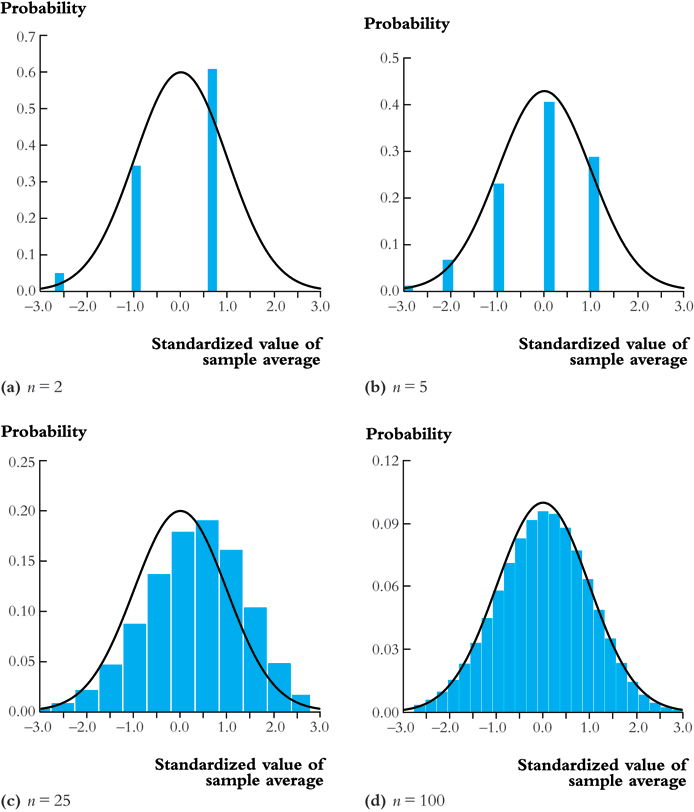
\includegraphics[width=0.8\textwidth]{figure/fig-2-9.png}
\caption{\label{fig:org19c79c6}
An illustration of the central limit theorem}
\end{figure}

Here is the demonstration of the CLT with Wolfram CDF Player,
\url{IllustratingTheCentralLimitTheoremWithSumsOfBernoulliRandomV.cdf}.
\end{document}